  \chapter{PENGUJIAN DAN ANALISIS}
\label{chap:pengujiananalisis}

% Ubah bagian-bagian berikut dengan isi dari pengujian dan analisis

Pada bab ini akan dipaparkan mengenai beberapa skenario pengujian sesuai dengan telah dijelaskan pada metodologi. Skenario pengujian ini dilakukan guna untuk mengetahui waktu \emph{delay} yang dibutuhkan untuk mentransmisikan data dari laptop menuju ESP32. Skenario yang nantinya akan diterapkan pada pengujian meliputi beberapa poin sebagai berikut:

\begin{enumerate}[nosep]
  \item Pengujian waktu \emph{delay} pengiriman data String melalui Bluetooth
  \item Pengujian waktu \emph{delay} pengiriman data JSON melalui Bluetooth
  \item Pengujian waktu \emph{delay} pengiriman data String melalui \emph{Access Point} WiFi
  \item Pengujian waktu \emph{delay} pengiriman data JSON melalui \emph{Access Point} WiFi
  \item Pengujian kestabilan Motor Kursi Roda
\end{enumerate}

Pelaksanaan metodologi serta skenario pengujian yang akan dipaparkan dalam bab ini diharapkan dapat memberikan pemahaman mengenai hasil dan pembahasan sehingga dapat ditarik kesimpulan dari Tugas Akhir yang telah dilaksanakan.


\section{Pengujian Waktu \emph{Delay} Pengiriman Data String Melalui Bluetooth}
\label{sec:delayBluetooth}

Pengujian waktu \emph{delay} pengiriman data ini dilakukan dengan cara mengirimkan data berupa string dari laptop menuju ESP32 melalui Bluetooth. Data yang dikirimkan adalah data arah dan kecepatan yang dipisahkan dengan koma seperti struktur data berikut ini \("Arah,Kecepatan"\).

Variabel arah memiliki tipe data \emph{char} yang digunakan untuk menentukan arah gerak dari motor kursi roda serta variabel kecepatan memiliki tipe data \emph{char} yang akan menentukan kecepatan maksimal dari rotasi motor kursi roda. Hasil dari pengujian waktu \emph{delay} pengiriman data string melalui bluetooth dapat dilihat pada Tabel \ref{tbl:delayBluetooth} dan Tabel \ref{tbl:delayBluetooth1}.

Tabel \ref{tbl:delayBluetooth} menampilkan pengiriman data string yang terdiri dari 2 nilai dan dipisahkan dengan simbol koma (","). Dalam pengujian kali ini, data dikirimkan sebanyak 30 kali secara berturut-turut. Setelah ESP32 menerima dan mengolah data maka Flag akan dikirimkan ke Laptop. Hal ini dilakukan agar ESP32 dapat menerima data dengan baik dan berhasil memisahkan dan memasukkan kedua nilai tersebut sesuai dengan variabel yang telah ditentukan. Hasil dari pengujian ini menunjukkan bahwa waktu pengiriman rata-rata dari laptop menuju ESP32 melalui Bluetooth adalah sebesar 1,037115767 detik.

Tabel \ref{tbl:delayBluetooth1} menampilkan pengiriman data string yang terdiri dari 1 nilai, yaitu arah. Dalam pengujian kali ini, data dikirimkan sebanyak 30 kali secara berturut-turut tanpa penambahan waktu \emph{delay} setiap kali mengirimkan data. Setelah ESP32 menerima dan mengolah data maka Flag akan dikirimkan ke Laptop. Hal ini dilakukan agar ESP32 dapat menerima data dengan baik dan berhasil memisahkan dan memasukkan kedua nilai tersebut sesuai dengan variabel yang telah ditentukan. Hasil dari pengujian ini menunjukkan bahwa waktu pengiriman rata-rata dari laptop menuju ESP32 melalui Bluetooth adalah sebesar 1,035209933 detik.

Ditemukan perbedaan waktu \emph{delay} yang tidak terlalu signifikan antara proses pengiriman string yang mengandung 2 nilai dibandingkan dengan string yang hanya berisi 1 nilai. Saat mengirimkan string yang memuat 2 data, pengujian menunjukkan adanya waktu \emph{delay} sekitar 1,037115767 detik. Dalam perbandingan dengan pengujian yang melibatkan string 1 nilai, waktu \emph{delay} yang tercatat hanya sekitar 1,035209933 detik. Setelah ESP32 menerima dan mengolah data maka Flag akan dikirimkan ke Laptop. Hal ini dilakukan agar ESP32 dapat menerima data secara optimal. Oleh karena itu, dapat disimpulkan bahwa dalam konteks pengiriman data melalui Bluetooth, pengguna dapat mengirim data string baik yang berisi 1 nilai maupun data string yang berisi 2 nilai, karena perbedaan waktu delay yang tidak terlalu berbeda.

% Tabel 4.1
\begin{table}[htpb]
  \centering
  \caption{Pengujian Waktu \emph{Delay} Pengiriman Data \emph{String} Berisi 2 Nilai Melalui Bluetooth}
  \label{tbl:delayBluetooth}
  \begin{tabular}{|ccc|c|}
  \hline
  \multicolumn{1}{|c|}{Data} & \multicolumn{1}{c|}{Timestamp Sent}  & Timestamp Received & Delay Time  \\ \hline
  \multicolumn{1}{|c|}{A,S}  & \multicolumn{1}{c|}{22:35:51.523626} & 22:35:52.588       & 1,064374    \\ \hline
  \multicolumn{1}{|c|}{E,T}  & \multicolumn{1}{c|}{22:35:52.552591} & 22:35:53.591       & 1,038409    \\ \hline
  \multicolumn{1}{|c|}{E,P}  & \multicolumn{1}{c|}{22:35:53.565132} & 22:35:54.610       & 1,044868    \\ \hline
  \multicolumn{1}{|c|}{B,S}  & \multicolumn{1}{c|}{22:35:54.579935} & 22:35:55.602       & 1,022065    \\ \hline
  \multicolumn{1}{|c|}{D,U}  & \multicolumn{1}{c|}{22:35:55.593733} & 22:35:56.619       & 1,025267    \\ \hline
  \multicolumn{1}{|c|}{C,P}  & \multicolumn{1}{c|}{22:35:56.609782} & 22:35:57.624       & 1,014218    \\ \hline
  \multicolumn{1}{|c|}{A,R}  & \multicolumn{1}{c|}{22:35:57.618772} & 22:35:58.666       & 1,047228    \\ \hline
  \multicolumn{1}{|c|}{D,Q}  & \multicolumn{1}{c|}{22:39:03.614853} & 22:39:04.672       & 1,057147    \\ \hline
  \multicolumn{1}{|c|}{C,O}  & \multicolumn{1}{c|}{22:39:04.651688} & 22:39:05.690       & 1,038312    \\ \hline
  \multicolumn{1}{|c|}{B,T}  & \multicolumn{1}{c|}{22:39:05.666397} & 22:39:06.679       & 1,012603    \\ \hline
  \multicolumn{1}{|c|}{B,S}  & \multicolumn{1}{c|}{22:39:06.676370} & 22:39:07.711       & 1,03463     \\ \hline
  \multicolumn{1}{|c|}{B,T}  & \multicolumn{1}{c|}{22:39:07.686293} & 22:39:08.724       & 1,037707    \\ \hline
  \multicolumn{1}{|c|}{B,T}  & \multicolumn{1}{c|}{22:39:08.692595} & 22:39:09.729       & 1,036405    \\ \hline
  \multicolumn{1}{|c|}{C,O}  & \multicolumn{1}{c|}{22:41:01.427643} & 22:41:02.485       & 1,057357    \\ \hline
  \multicolumn{1}{|c|}{D,U}  & \multicolumn{1}{c|}{22:41:02.443022} & 22:41:03.486       & 1,042978    \\ \hline
  \multicolumn{1}{|c|}{A,U}  & \multicolumn{1}{c|}{22:41:03.449566} & 22:41:04.485       & 1,035434    \\ \hline
  \multicolumn{1}{|c|}{B,O}  & \multicolumn{1}{c|}{22:41:04.463072} & 22:41:05.507       & 1,043928    \\ \hline
  \multicolumn{1}{|c|}{D,O}  & \multicolumn{1}{c|}{22:41:05.470721} & 22:41:06.493       & 1,022279    \\ \hline
  \multicolumn{1}{|c|}{C,T}  & \multicolumn{1}{c|}{22:41:06.477458} & 22:41:07.512       & 1,034542    \\ \hline
  \multicolumn{1}{|c|}{B,U}  & \multicolumn{1}{c|}{22:41:07.492309} & 22:41:08.516       & 1,023691    \\ \hline
  \multicolumn{1}{|c|}{D,R}  & \multicolumn{1}{c|}{22:41:08.499671} & 22:41:09.532       & 1,032329    \\ \hline
  \multicolumn{1}{|c|}{E,Q}  & \multicolumn{1}{c|}{22:41:09.509928} & 22:41:10.547       & 1,037072    \\ \hline
  \multicolumn{1}{|c|}{E,V}  & \multicolumn{1}{c|}{22:41:10.523644} & 22:41:11.563       & 1,039356    \\ \hline
  \multicolumn{1}{|c|}{C,U}  & \multicolumn{1}{c|}{22:43:11.001438} & 22:43:12.026       & 1,024562    \\ \hline
  \multicolumn{1}{|c|}{C,P}  & \multicolumn{1}{c|}{22:43:12.028891} & 22:43:13.072       & 1,043109    \\ \hline
  \multicolumn{1}{|c|}{A,T}  & \multicolumn{1}{c|}{22:43:13.035252} & 22:43:14.066       & 1,030748    \\ \hline
  \multicolumn{1}{|c|}{D,Q}  & \multicolumn{1}{c|}{22:43:14.044212} & 22:43:15.086       & 1,041788    \\ \hline
  \multicolumn{1}{|c|}{D,O}  & \multicolumn{1}{c|}{22:43:15.050093} & 22:43:16.087       & 1,036907    \\ \hline
  \multicolumn{1}{|c|}{C,V}  & \multicolumn{1}{c|}{22:44:38.377450} & 22:44:39.438       & 1,06055     \\ \hline
  \multicolumn{1}{|c|}{B,P}  & \multicolumn{1}{c|}{22:44:39.427390} & 22:44:40.461       & 1,03361     \\ \hline
  \multicolumn{3}{|c|}{Average Delay Time}                                               & 1,037115767 \\ \hline
  \end{tabular}
  \end{table}

% Tabel 4.2
\begin{table}[htpb]
  \centering
  \caption{Pengujian Waktu \emph{Delay} Pengiriman Data \emph{String} Berisi 1 Nilai Melalui Bluetooth}
  \label{tbl:delayBluetooth1}
  \begin{tabular}{|ccc|c|}
  \hline
  \multicolumn{1}{|c|}{Data} & \multicolumn{1}{c|}{Timestamp Sent}  & Timestamp Received & Delay Time  \\ \hline
  \multicolumn{1}{|c|}{B}    & \multicolumn{1}{c|}{22:17:58.360200} & 22:17:59.417       & 1,0568      \\ \hline
  \multicolumn{1}{|c|}{B}    & \multicolumn{1}{c|}{22:17:59.396644} & 22:18:00.426       & 1,029356    \\ \hline
  \multicolumn{1}{|c|}{B}    & \multicolumn{1}{c|}{22:18:00.411642} & 22:18:01.449       & 1,037358    \\ \hline
  \multicolumn{1}{|c|}{C}    & \multicolumn{1}{c|}{22:18:01.419172} & 22:18:02.461       & 1,041828    \\ \hline
  \multicolumn{1}{|c|}{E}    & \multicolumn{1}{c|}{22:18:02.431706} & 22:18:03.436       & 1,004294    \\ \hline
  \multicolumn{1}{|c|}{B}    & \multicolumn{1}{c|}{22:18:03.441714} & 22:18:04.487       & 1,045286    \\ \hline
  \multicolumn{1}{|c|}{A}    & \multicolumn{1}{c|}{22:18:04.452937} & 22:18:05.481       & 1,028063    \\ \hline
  \multicolumn{1}{|c|}{B}    & \multicolumn{1}{c|}{22:18:05.468058} & 22:18:06.502       & 1,033942    \\ \hline
  \multicolumn{1}{|c|}{C}    & \multicolumn{1}{c|}{22:18:06.475522} & 22:18:07.504       & 1,028478    \\ \hline
  \multicolumn{1}{|c|}{A}    & \multicolumn{1}{c|}{22:18:07.483055} & 22:18:08.508       & 1,024945    \\ \hline
  \multicolumn{1}{|c|}{C}    & \multicolumn{1}{c|}{22:19:35.549304} & 22:19:36.610       & 1,060696    \\ \hline
  \multicolumn{1}{|c|}{A}    & \multicolumn{1}{c|}{22:19:36.580394} & 22:19:37.624       & 1,043606    \\ \hline
  \multicolumn{1}{|c|}{B}    & \multicolumn{1}{c|}{22:19:37.587334} & 22:19:38.612       & 1,024666    \\ \hline
  \multicolumn{1}{|c|}{B}    & \multicolumn{1}{c|}{22:19:38.593528} & 22:19:39.645       & 1,051472    \\ \hline
  \multicolumn{1}{|c|}{E}    & \multicolumn{1}{c|}{22:19:39.605674} & 22:19:40.634       & 1,028326    \\ \hline
  \multicolumn{1}{|c|}{E}    & \multicolumn{1}{c|}{22:19:40.621872} & 22:19:41.643       & 1,021128    \\ \hline
  \multicolumn{1}{|c|}{A}    & \multicolumn{1}{c|}{22:19:41.633767} & 22:19:42.668       & 1,034233    \\ \hline
  \multicolumn{1}{|c|}{D}    & \multicolumn{1}{c|}{22:19:42.641717} & 22:19:43.675       & 1,033283    \\ \hline
  \multicolumn{1}{|c|}{E}    & \multicolumn{1}{c|}{22:19:43.650596} & 22:19:44.682       & 1,031404    \\ \hline
  \multicolumn{1}{|c|}{D}    & \multicolumn{1}{c|}{22:19:44.659460} & 22:19:45.698       & 1,03854     \\ \hline
  \multicolumn{1}{|c|}{A}    & \multicolumn{1}{c|}{22:20:22.820901} & 22:20:23.885       & 1,064099    \\ \hline
  \multicolumn{1}{|c|}{E}    & \multicolumn{1}{c|}{22:20:23.850953} & 22:20:24.900       & 1,049047    \\ \hline
  \multicolumn{1}{|c|}{B}    & \multicolumn{1}{c|}{22:20:24.867989} & 22:20:25.873       & 1,005011    \\ \hline
  \multicolumn{1}{|c|}{E}    & \multicolumn{1}{c|}{22:20:25.879869} & 22:20:26.919       & 1,039131    \\ \hline
  \multicolumn{1}{|c|}{C}    & \multicolumn{1}{c|}{22:20:26.890743} & 22:20:27.925       & 1,034257    \\ \hline
  \multicolumn{1}{|c|}{D}    & \multicolumn{1}{c|}{22:20:27.899877} & 22:20:28.944       & 1,044123    \\ \hline
  \multicolumn{1}{|c|}{B}    & \multicolumn{1}{c|}{22:20:28.911163} & 22:20:29.917       & 1,005837    \\ \hline
  \multicolumn{1}{|c|}{A}    & \multicolumn{1}{c|}{22:20:29.918844} & 22:20:30.969       & 1,050156    \\ \hline
  \multicolumn{1}{|c|}{E}    & \multicolumn{1}{c|}{22:20:30.945381} & 22:20:31.991       & 1,045619    \\ \hline
  \multicolumn{1}{|c|}{E}    & \multicolumn{1}{c|}{22:20:31.972686} & 22:20:32.994       & 1,021314    \\ \hline
  \multicolumn{3}{|c|}{Average Delay Time}                                               & 1,035209933 \\ \hline
  \end{tabular}
  \end{table}

\newpage

\section{Pengujian Waktu \emph{Delay} Pengiriman Data JSON Melalui Bluetooth}
\label{sec:delayBluetoothJSON}

Pengujian waktu \emph{delay} pengiriman data ini dilakukan dengan cara mengirimkan data berupa JSON dari laptop menuju ESP32 melalui Bluetooth. Data yang dikirimkan adalah data arah dan kecepatan yang dirangkum menjadi JSON seperti struktur berikut \(\{'arah': kode-arah, 'kecepatan': level-kecepatan\}\) 

Data JSON terdiri dari 2 bagian, yaitu \emph{key} dan \emph{value}. Terdapat 2 \emph{key}, yaitu arah dan kecepatan. \emph{Key} arah berisi \emph{value} dengan tipe data char yang digunakan untuk menentukan arah gerak dari motor kursi roda dan \emph{key} kecepatan berisi \emph{value} dengan tipe data \emph{char} yang digunakan untuk menentukan kecepatan maksimal dari rotasi motor kursi roda. Hasil dari pengujian waktu \emph{delay} pengiriman data JSON dapat dilihat pada Tabel \ref{tbl:delayBluetoothJSON2} dan Tabel \ref{tbl:delayBluetoothJSON1}.

Tabel \ref{tbl:delayBluetoothJSON2} menampilkan pengiriman JSON yang terdiri dari 2 \emph{key}-\emph{value}, yaitu arah dan kecepatan. Dalam pengujian kali ini, data dikirimkan sebanyak 29 kali secara berturut-turut. Setelah ESP32 menerima dan mengolah data maka Flag akan dikirimkan ke Laptop. Hal ini dilakukan agar ESP32 dapat menerima data dengan baik dan berhasil memisahkan (\emph{deserialize}) serta memasukkan kedua nilai tersebut sesuai dengan variabel yang telah ditentukan. Hasil dari pengujian ini menunjukkan bahwa waktu pengiriman rata-rata dari laptop menuju ESP32 melalui Bluetooth adalah sebesar 1,038895345 detik.

Tabel \ref{tbl:delayBluetoothJSON1} menampilkan pengiriman JSON yang terdiri dari 1 \emph{key}-\emph{value}, yaitu arah. Dalam pengujian kali ini, data dikirimkan sebanyak 44 kali secara berturut-turut. Setelah ESP32 menerima dan mengolah data maka Flag akan dikirimkan ke Laptop. Hal ini dilakukan agar ESP32 dapat menerima data dengan baik dan berhasil memisahkan (\emph{deserialize}) serta memasukkan nilai tersebut sesuai dengan variabel yang telah ditentukan. Hasil dari pengujian ini menunjukkan waktu pengiriman rata-rata dari laptop menuju ESP32 melalui Bluetooth sebesar 1,033746386 detik.

Dari kedua cara pengujian tersebut, didapatkan bahwa waktu \emph{delay} antara proses pengiriman JSON yang mengandung 2 \emph{key}-\emph{value} dibandingkan dengan JSON yang hanya berisikan 1 \emph{key}-\emph{value} tidak terlalu signifikan. Saat mengirimkan JSON yang berisikan 2 \emph{key}-\emph{value}, pengujian menunjukkan adanya \emph{delay} sebesar 1,038895345 detik. Jika dibandingkan dengan pengujian yang mengirimkan JSON dengan 1 \emph{key}-\emph{value}, waktu \emph{delay} yang tercatat adalah sebesar 1,033746386 detik. Dapat disimpulkan bahwa dalam konteks pengiriman data melalui Bluetooth, maka pengguna dapat mengirimkan data JSON baik yang berisi 1 \emph{key}-\emph{value} maupun yang berisi 2 \emph{key}-\emph{value}, karena perbedaan \emph{delay} kedua teknik tersebut tidak terlalu signifikan.

% Tabel 4.3
\begin{table}[htpb]
  \centering
  \caption{Pengujian Waktu \emph{Delay} Pengiriman Data JSON Berisi 2 Nilai Melalui Bluetooth}
  \label{tbl:delayBluetoothJSON2}
  \begin{tabular}{|ccc|c|}
  \hline
  \multicolumn{1}{|c|}{Data}                              & \multicolumn{1}{c|}{Timestamp Sent}  & Timestamp Received & Delay Time  \\ \hline
  \multicolumn{1}{|c|}{\{'arah': 'A', 'kecepatan': 'W'\}} & \multicolumn{1}{c|}{00:15:50.714083} & 00:15:51.776       & 1,061917    \\ \hline
  \multicolumn{1}{|c|}{\{"arah": "D", "kecepatan": "T"\}} & \multicolumn{1}{c|}{00:15:51.747698} & 00:15:52.796       & 1,048302    \\ \hline
  \multicolumn{1}{|c|}{\{"arah": "E", "kecepatan": "S"\}} & \multicolumn{1}{c|}{00:15:52.756331} & 00:15:53.766       & 1,009669    \\ \hline
  \multicolumn{1}{|c|}{\{"arah": "D", "kecepatan": "V"\}} & \multicolumn{1}{c|}{00:15:53.768717} & 00:15:54.807       & 1,038283    \\ \hline
  \multicolumn{1}{|c|}{\{"arah": "B", "kecepatan": "W"\}} & \multicolumn{1}{c|}{00:15:54.784688} & 00:15:55.824       & 1,039312    \\ \hline
  \multicolumn{1}{|c|}{\{"arah": "D", "kecepatan": "Q"\}} & \multicolumn{1}{c|}{00:15:55.792741} & 00:15:56.841       & 1,048259    \\ \hline
  \multicolumn{1}{|c|}{\{"arah": "A", "kecepatan": "O"\}} & \multicolumn{1}{c|}{00:15:56.803679} & 00:15:57.848       & 1,044321    \\ \hline
  \multicolumn{1}{|c|}{\{"arah": "E", "kecepatan": "Q"\}} & \multicolumn{1}{c|}{00:15:57.809707} & 00:15:58.854       & 1,044293    \\ \hline
  \multicolumn{1}{|c|}{\{"arah": "A", "kecepatan": "T"\}} & \multicolumn{1}{c|}{00:15:58.828668} & 00:15:59.840       & 1,011332    \\ \hline
  \multicolumn{1}{|c|}{\{"arah": "B", "kecepatan": "U"\}} & \multicolumn{1}{c|}{00:15:59.837626} & 00:16:00.875       & 1,037374    \\ \hline
  \multicolumn{1}{|c|}{\{"arah": "A", "kecepatan": "V"\}} & \multicolumn{1}{c|}{00:16:00.852674} & 00:16:01.888       & 1,035326    \\ \hline
  \multicolumn{1}{|c|}{\{"arah": "C", "kecepatan": "Q"\}} & \multicolumn{1}{c|}{00:16:01.867249} & 00:16:02.895       & 1,027751    \\ \hline
  \multicolumn{1}{|c|}{\{"arah": "A", "kecepatan": "O"\}} & \multicolumn{1}{c|}{00:16:02.885202} & 00:16:03.932       & 1,046798    \\ \hline
  \multicolumn{1}{|c|}{\{"arah": "A", "kecepatan": "V"\}} & \multicolumn{1}{c|}{00:16:03.910200} & 00:16:04.953       & 1,0428      \\ \hline
  \multicolumn{1}{|c|}{\{"arah": "B", "kecepatan": "T"\}} & \multicolumn{1}{c|}{00:16:04.917273} & 00:16:05.962       & 1,044727    \\ \hline
  \multicolumn{1}{|c|}{\{"arah": "D", "kecepatan": "W"\}} & \multicolumn{1}{c|}{00:16:05.925647} & 00:16:06.947       & 1,021353    \\ \hline
  \multicolumn{1}{|c|}{\{"arah": "E", "kecepatan": "P"\}} & \multicolumn{1}{c|}{00:16:06.942693} & 00:16:07.981       & 1,038307    \\ \hline
  \multicolumn{1}{|c|}{\{"arah": "E", "kecepatan": "R"\}} & \multicolumn{1}{c|}{00:16:07.955136} & 00:16:09.004       & 1,048864    \\ \hline
  \multicolumn{1}{|c|}{\{"arah": "A", "kecepatan": "T"\}} & \multicolumn{1}{c|}{00:16:08.966673} & 00:16:10.013       & 1,046327    \\ \hline
  \multicolumn{1}{|c|}{\{"arah": "E", "kecepatan": "P"\}} & \multicolumn{1}{c|}{00:16:09.977653} & 00:16:11.029       & 1,051347    \\ \hline
  \multicolumn{1}{|c|}{\{"arah": "E", "kecepatan": "O"\}} & \multicolumn{1}{c|}{00:16:10.985241} & 00:16:12.033       & 1,047759    \\ \hline
  \multicolumn{1}{|c|}{\{"arah": "C", "kecepatan": "R"\}} & \multicolumn{1}{c|}{00:16:11.997910} & 00:16:13.010       & 1,01209     \\ \hline
  \multicolumn{1}{|c|}{\{'arah': 'A', 'kecepatan': 'V'\}} & \multicolumn{1}{c|}{02:33:35.225933} & 02:33:36.305       & 1,079067    \\ \hline
  \multicolumn{1}{|c|}{\{"arah": "D", "kecepatan": "U"\}} & \multicolumn{1}{c|}{02:33:36.263807} & 02:33:37.288       & 1,024193    \\ \hline
  \multicolumn{1}{|c|}{\{"arah": "A", "kecepatan": "R"\}} & \multicolumn{1}{c|}{02:33:37.274213} & 02:33:38.297       & 1,022787    \\ \hline
  \multicolumn{1}{|c|}{\{"arah": "C", "kecepatan": "W"\}} & \multicolumn{1}{c|}{02:33:38.309262} & 02:33:39.356       & 1,046738    \\ \hline
  \multicolumn{1}{|c|}{\{"arah": "B", "kecepatan": "U"\}} & \multicolumn{1}{c|}{02:33:39.324412} & 02:33:40.382       & 1,057588    \\ \hline
  \multicolumn{1}{|c|}{\{"arah": "A", "kecepatan": "O"\}} & \multicolumn{1}{c|}{02:33:40.394353} & 02:33:41.424       & 1,029647    \\ \hline
  \multicolumn{1}{|c|}{\{"arah": "B", "kecepatan": "T"\}} & \multicolumn{1}{c|}{02:33:41.411566} & 02:33:42.433       & 1,021434    \\ \hline
  \multicolumn{3}{|c|}{Average Delay Time}                                                                            & 1,038895345 \\ \hline
  \end{tabular}
  \end{table}

% Tabel 4.4
\begin{table}[htpb]
  \centering
  \caption{Pengujian Waktu \emph{Delay} Pengiriman Data JSON Berisi 1 Nilai Melalui Bluetooth}
  \label{tbl:delayBluetoothJSON1}
  \begin{tabular}{|ccc|c|}
  \hline
  \multicolumn{1}{|c|}{Data}            & \multicolumn{1}{c|}{Timestamp Sent}  & Timestamp Received & Delay Time  \\ \hline
  \multicolumn{1}{|c|}{\{'arah': 'D'\}} & \multicolumn{1}{c|}{23:51:13.043594} & 23:51:14.086       & 1,042406    \\ \hline
  \multicolumn{1}{|c|}{\{"arah": "A"\}} & \multicolumn{1}{c|}{23:51:14.076700} & 23:51:15.105       & 1,0283      \\ \hline
  \multicolumn{1}{|c|}{\{"arah": "D"\}} & \multicolumn{1}{c|}{23:51:15.086795} & 23:51:16.117       & 1,030205    \\ \hline
  \multicolumn{1}{|c|}{\{"arah": "E"\}} & \multicolumn{1}{c|}{23:51:16.099483} & 23:51:17.140       & 1,040517    \\ \hline
  \multicolumn{1}{|c|}{\{"arah": "C"\}} & \multicolumn{1}{c|}{23:51:17.105868} & 23:51:18.149       & 1,043132    \\ \hline
  \multicolumn{1}{|c|}{\{"arah": "C"\}} & \multicolumn{1}{c|}{23:51:18.117818} & 23:51:19.166       & 1,048182    \\ \hline
  \multicolumn{1}{|c|}{\{"arah": "E"\}} & \multicolumn{1}{c|}{23:51:19.127469} & 23:51:20.146       & 1,018531    \\ \hline
  \multicolumn{1}{|c|}{\{"arah": "B"\}} & \multicolumn{1}{c|}{23:51:20.135577} & 23:51:21.166       & 1,030423    \\ \hline
  \multicolumn{1}{|c|}{\{"arah": "C"\}} & \multicolumn{1}{c|}{23:51:21.145479} & 23:51:22.190       & 1,044521    \\ \hline
  \multicolumn{1}{|c|}{\{"arah": "C"\}} & \multicolumn{1}{c|}{23:51:22.158915} & 23:51:23.176       & 1,017085    \\ \hline
  \multicolumn{1}{|c|}{\{"arah": "E"\}} & \multicolumn{1}{c|}{23:51:23.168461} & 23:51:24.180       & 1,011539    \\ \hline
  \multicolumn{1}{|c|}{\{"arah": "D"\}} & \multicolumn{1}{c|}{23:51:24.180958} & 23:51:25.207       & 1,026042    \\ \hline
  \multicolumn{1}{|c|}{\{"arah": "A"\}} & \multicolumn{1}{c|}{23:51:25.194500} & 23:51:26.199       & 1,0045      \\ \hline
  \multicolumn{1}{|c|}{\{"arah": "C"\}} & \multicolumn{1}{c|}{23:51:26.203449} & 23:51:27.244       & 1,040551    \\ \hline
  \multicolumn{1}{|c|}{\{"arah": "A"\}} & \multicolumn{1}{c|}{23:51:27.216460} & 23:51:28.254       & 1,03754     \\ \hline
  \multicolumn{1}{|c|}{\{"arah": "A"\}} & \multicolumn{1}{c|}{23:51:28.224202} & 23:51:29.260       & 1,035798    \\ \hline
  \multicolumn{1}{|c|}{\{"arah": "C"\}} & \multicolumn{1}{c|}{23:51:29.236461} & 23:51:30.280       & 1,043539    \\ \hline
  \multicolumn{1}{|c|}{\{"arah": "A"\}} & \multicolumn{1}{c|}{23:51:30.243411} & 23:51:31.287       & 1,043589    \\ \hline
  \multicolumn{1}{|c|}{\{"arah": "D"\}} & \multicolumn{1}{c|}{23:51:31.253768} & 23:51:32.293       & 1,039232    \\ \hline
  \multicolumn{1}{|c|}{\{"arah": "A"\}} & \multicolumn{1}{c|}{23:51:32.266472} & 23:51:33.301       & 1,034528    \\ \hline
  \multicolumn{1}{|c|}{\{"arah": "C"\}} & \multicolumn{1}{c|}{23:51:33.279736} & 23:51:34.327       & 1,047264    \\ \hline
  \multicolumn{1}{|c|}{\{"arah": "D"\}} & \multicolumn{1}{c|}{23:51:34.288698} & 23:51:35.332       & 1,043302    \\ \hline
  \multicolumn{1}{|c|}{\{"arah": "C"\}} & \multicolumn{1}{c|}{23:51:35.303347} & 23:51:36.345       & 1,041653    \\ \hline
  \multicolumn{1}{|c|}{\{"arah": "E"\}} & \multicolumn{1}{c|}{23:51:36.323448} & 23:51:37.351       & 1,027552    \\ \hline
  \multicolumn{1}{|c|}{\{"arah": "E"\}} & \multicolumn{1}{c|}{23:51:37.331450} & 23:51:38.357       & 1,02555     \\ \hline
  \multicolumn{1}{|c|}{\{"arah": "C"\}} & \multicolumn{1}{c|}{23:51:38.341408} & 23:51:39.383       & 1,041592    \\ \hline
  \multicolumn{1}{|c|}{\{"arah": "A"\}} & \multicolumn{1}{c|}{23:51:39.351443} & 23:51:40.356       & 1,004557    \\ \hline
  \multicolumn{1}{|c|}{\{"arah": "B"\}} & \multicolumn{1}{c|}{23:51:40.366713} & 23:51:41.412       & 1,045287    \\ \hline
  \multicolumn{1}{|c|}{\{"arah": "D"\}} & \multicolumn{1}{c|}{23:51:41.377986} & 23:51:42.415       & 1,037014    \\ \hline
  \multicolumn{1}{|c|}{\{"arah": "E"\}} & \multicolumn{1}{c|}{23:51:42.392035} & 23:51:43.421       & 1,028965    \\ \hline
  \multicolumn{1}{|c|}{\{"arah": "B"\}} & \multicolumn{1}{c|}{23:51:43.406513} & 23:51:44.431       & 1,024487    \\ \hline
  \multicolumn{1}{|c|}{\{"arah": "C"\}} & \multicolumn{1}{c|}{23:51:44.424451} & 23:51:45.464       & 1,039549    \\ \hline
  \multicolumn{1}{|c|}{\{"arah": "C"\}} & \multicolumn{1}{c|}{23:51:45.430967} & 23:51:46.477       & 1,046033    \\ \hline
  \multicolumn{1}{|c|}{\{"arah": "C"\}} & \multicolumn{1}{c|}{23:51:46.438140} & 23:51:47.486       & 1,04786     \\ \hline
  \multicolumn{1}{|c|}{\{"arah": "B"\}} & \multicolumn{1}{c|}{23:51:47.449801} & 23:51:48.476       & 1,026199    \\ \hline
  \multicolumn{1}{|c|}{\{"arah": "C"\}} & \multicolumn{1}{c|}{23:51:48.457089} & 23:51:49.496       & 1,038911    \\ \hline
  \multicolumn{1}{|c|}{\{"arah": "E"\}} & \multicolumn{1}{c|}{23:51:49.471782} & 23:51:50.496       & 1,024218    \\ \hline
  \multicolumn{1}{|c|}{\{"arah": "B"\}} & \multicolumn{1}{c|}{23:51:50.487487} & 23:51:51.525       & 1,037513    \\ \hline
  \multicolumn{1}{|c|}{\{"arah": "D"\}} & \multicolumn{1}{c|}{23:51:51.496917} & 23:51:52.538       & 1,041083    \\ \hline
  \multicolumn{1}{|c|}{\{"arah": "D"\}} & \multicolumn{1}{c|}{23:51:52.504746} & 23:51:53.528       & 1,023254    \\ \hline
  \multicolumn{1}{|c|}{\{"arah": "B"\}} & \multicolumn{1}{c|}{23:51:53.519392} & 23:51:54.569       & 1,049608    \\ \hline
  \multicolumn{1}{|c|}{\{"arah": "D"\}} & \multicolumn{1}{c|}{23:51:54.526676} & 23:51:55.555       & 1,028324    \\ \hline
  \multicolumn{1}{|c|}{\{"arah": "B"\}} & \multicolumn{1}{c|}{23:51:55.539415} & 23:51:56.571       & 1,031585    \\ \hline
  \multicolumn{1}{|c|}{\{"arah": "E"\}} & \multicolumn{1}{c|}{23:51:56.552679} & 23:51:57.576       & 1,023321    \\ \hline
  \multicolumn{3}{|c|}{Average Delay Time}                                                          & 1,033746386 \\ \hline
  \end{tabular}
\end{table}

\newpage

\section{Pengujian Waktu \emph{Delay} Pengiriman Data String Melalui \emph{Access Point} WiFi}
\label{sec:delayWiFi}

Pengujian waktu \emph{delay} pengiriman data ini dilakukan dengan cara mengirimkan data berupa String dari laptop menuji ESP32 melalui WiFi. ESP32 diatur sebagai \emph{Access Point}. Data yang dikirimkan adalah data arah dan kecepatan yang dipisahkan dengan simbol koma seperti struktur data berikut ini \("Arah, Kecepatan"\).

Variabel arah memiliki tipe data \emph{char} yang digunakan untuk menentukan arah gerak dari motor kursi roda serta variabel kecepatan yang memiliki tipe data \emph{char} yang akan menentukan kecepatan maksimal dari rotasi motor kursi roda. Hasil dari pengujian waktu \emph{delay} pengiriman data String melalui WiFi dapat dilihat pada Tabel \ref{tbl:delayWiFi2} dan Tabel \ref{tbl:delayWiFi1}

Tabel \ref{tbl:delayWiFi2} menampilkan pengiriman data string yang terdiri dari 2 nilai dan dipisahkan dengan simbol koma (","). Dalam pengujian kali ini, data dikirimkan sebanyak 33 kali secara berturut-turut. Setelah ESP32 menerima dan mengolah data maka Flag akan dikirimkan ke Laptop. Hal ini dilakukan agar ESP32 dapat menerima data dengan baik dan berhasil memisahkan dan memasukkan kedua nilai tersebut sesuai dengan variabel yang telah ditentukan. Hasil dari pengujian ini menunjukkan bahwa waktu pengiriman rata-rata dari laptop menuju ESP32 melalui WiFi adalah sebesar 1,035478061 detik.

Tabel \ref{tbl:delayWiFi1} menampilkan pengiriman data string yang terdiri dari 1 nilai, yaitu arah. Dalam pengujian kali ini, data dikirimkan sebanyak 32 kali secara berturut-turut. Setelah ESP32 menerima dan mengolah data maka Flag akan dikirimkan ke Laptop. Hasil dari pengujian ini menunjukkan bahwa waktu pengiriman rata-rata dari laptop menuju ESP32 melalui WiFi adalah sebesar 1,03470275 detik.

Ditemukan perbedaan waktu \emph{delay} yang tidak terlalu signifikan antara proses pengiriman string yang mengandung 2 nilai dibandingkan dengan string yang hanya berisikan 1 nilai. Saat mengirimkan string yang memuat 2 data, pengujian menunjukkan adanya waktu \emph{delay} sekitar 1,035478061 detik. Dalam perbandingan dengan pengujian yang melibatkan string dengan 1 nilai, waktu \emph{delay} yang tercatat sebesar 1,03470275 detik. Setelah ESP32 menerima dan mengolah data maka Flag akan dikirimkan ke Laptop. Hal ini dilakukan agar ESP32 dapat menerima data secara optimal. Oleh karena itu, dapat disimpulkan bahwa dalam konteks pengiriman data melalui WiFi, pengguna dapat mengirimkan data string baik yang berisi 1 nilai maupun data string dengan 2 nilai, karena perbedaan waktu \emph{delay} yang tidak terlalu signifikan.

% Tabel 4.5
\begin{table}[htpb]
  \centering
  \caption{Pengujian Waktu \emph{Delay} Pengiriman Data \emph{String} Berisi 2 Nilai Melalui \emph{Access Point} WiFi}
  \label{tbl:delayWiFi2}
  \begin{tabular}{|ccc|c|}
  \hline
  \multicolumn{1}{|c|}{Data} & \multicolumn{1}{c|}{Timestamp Sent}  & Timestamp Received & Delay Time  \\ \hline
  \multicolumn{1}{|c|}{A,Q}  & \multicolumn{1}{c|}{03:49:59.217022} & 03:50:00.256       & 1,038978    \\ \hline
  \multicolumn{1}{|c|}{D,S}  & \multicolumn{1}{c|}{03:50:00.232977} & 03:50:01.260       & 1,027023    \\ \hline
  \multicolumn{1}{|c|}{A,O}  & \multicolumn{1}{c|}{03:50:01.256289} & 03:50:02.301       & 1,044711    \\ \hline
  \multicolumn{1}{|c|}{B,Q}  & \multicolumn{1}{c|}{03:50:02.278635} & 03:50:03.317       & 1,038365    \\ \hline
  \multicolumn{1}{|c|}{A,P}  & \multicolumn{1}{c|}{03:50:03.303124} & 03:50:04.336       & 1,032876    \\ \hline
  \multicolumn{1}{|c|}{E,U}  & \multicolumn{1}{c|}{03:50:04.326652} & 03:50:05.374       & 1,047348    \\ \hline
  \multicolumn{1}{|c|}{B,U}  & \multicolumn{1}{c|}{03:50:05.365324} & 03:50:06.411       & 1,045676    \\ \hline
  \multicolumn{1}{|c|}{D,R}  & \multicolumn{1}{c|}{03:50:06.374651} & 03:50:07.413       & 1,038349    \\ \hline
  \multicolumn{1}{|c|}{B,U}  & \multicolumn{1}{c|}{03:50:07.403115} & 03:50:08.432       & 1,028885    \\ \hline
  \multicolumn{1}{|c|}{E,Q}  & \multicolumn{1}{c|}{03:50:08.422259} & 03:50:09.469       & 1,046741    \\ \hline
  \multicolumn{1}{|c|}{D,S}  & \multicolumn{1}{c|}{03:50:09.452763} & 03:50:10.486       & 1,033237    \\ \hline
  \multicolumn{1}{|c|}{A,Q}  & \multicolumn{1}{c|}{03:50:10.470206} & 03:50:11.489       & 1,018794    \\ \hline
  \multicolumn{1}{|c|}{B,V}  & \multicolumn{1}{c|}{03:50:11.513787} & 03:50:12.556       & 1,042213    \\ \hline
  \multicolumn{1}{|c|}{D,S}  & \multicolumn{1}{c|}{03:50:12.519142} & 03:50:13.559       & 1,039858    \\ \hline
  \multicolumn{1}{|c|}{B,U}  & \multicolumn{1}{c|}{03:50:13.547184} & 03:50:14.595       & 1,047816    \\ \hline
  \multicolumn{1}{|c|}{C,S}  & \multicolumn{1}{c|}{03:50:14.566997} & 03:50:15.588       & 1,021003    \\ \hline
  \multicolumn{1}{|c|}{D,R}  & \multicolumn{1}{c|}{03:50:15.600210} & 03:50:16.638       & 1,03779     \\ \hline
  \multicolumn{1}{|c|}{C,W}  & \multicolumn{1}{c|}{03:50:16.616353} & 03:50:17.645       & 1,028647    \\ \hline
  \multicolumn{1}{|c|}{E,O}  & \multicolumn{1}{c|}{03:50:17.628725} & 03:50:18.664       & 1,035275    \\ \hline
  \multicolumn{1}{|c|}{C,Q}  & \multicolumn{1}{c|}{03:50:18.640125} & 03:50:19.654       & 1,013875    \\ \hline
  \multicolumn{1}{|c|}{D,U}  & \multicolumn{1}{c|}{03:50:19.645720} & 03:50:20.695       & 1,04928     \\ \hline
  \multicolumn{1}{|c|}{E,T}  & \multicolumn{1}{c|}{03:50:20.652242} & 03:50:21.674       & 1,021758    \\ \hline
  \multicolumn{1}{|c|}{A,S}  & \multicolumn{1}{c|}{03:50:21.664690} & 03:50:22.708       & 1,04331     \\ \hline
  \multicolumn{1}{|c|}{B,T}  & \multicolumn{1}{c|}{03:50:22.668332} & 03:50:23.705       & 1,036668    \\ \hline
  \multicolumn{1}{|c|}{E,P}  & \multicolumn{1}{c|}{03:50:23.671113} & 03:50:24.716       & 1,044887    \\ \hline
  \multicolumn{1}{|c|}{E,S}  & \multicolumn{1}{c|}{03:50:24.677001} & 03:50:25.719       & 1,041999    \\ \hline
  \multicolumn{1}{|c|}{A,V}  & \multicolumn{1}{c|}{03:50:25.683752} & 03:50:26.717       & 1,033248    \\ \hline
  \multicolumn{1}{|c|}{E,U}  & \multicolumn{1}{c|}{03:50:26.692210} & 03:50:27.719       & 1,02679     \\ \hline
  \multicolumn{1}{|c|}{C,V}  & \multicolumn{1}{c|}{03:50:27.696829} & 03:50:28.738       & 1,041171    \\ \hline
  \multicolumn{1}{|c|}{C,U}  & \multicolumn{1}{c|}{03:50:28.715728} & 03:50:29.738       & 1,022272    \\ \hline
  \multicolumn{1}{|c|}{D,R}  & \multicolumn{1}{c|}{03:50:29.719687} & 03:50:30.740       & 1,020313    \\ \hline
  \multicolumn{1}{|c|}{B,U}  & \multicolumn{1}{c|}{03:50:30.725229} & 03:50:31.760       & 1,034771    \\ \hline
  \multicolumn{1}{|c|}{B,R}  & \multicolumn{1}{c|}{03:50:31.731151} & 03:50:32.778       & 1,046849    \\ \hline
  \multicolumn{3}{|c|}{Average Delay Time}                                               & 1,035478061 \\ \hline
  \end{tabular}
\end{table}

% Tabel 4.6
\begin{table}[htpb]
\centering
  \caption{Pengujian Waktu \emph{Delay} Pengiriman Data \emph{String} Berisi 1 Nilai Melalui \emph{Access Point} WiFi}
  \label{tbl:delayWiFi1}
  \begin{tabular}{|ccc|c|}
  \hline
  \multicolumn{1}{|c|}{Data} & \multicolumn{1}{c|}{Timestamp Sent}  & Timestamp Received & Delay Time \\ \hline
  \multicolumn{1}{|c|}{C}    & \multicolumn{1}{c|}{03:40:01.384466} & 03:40:02.417       & 1,032534   \\ \hline
  \multicolumn{1}{|c|}{B}    & \multicolumn{1}{c|}{03:40:02.390604} & 03:40:03.432       & 1,041396   \\ \hline
  \multicolumn{1}{|c|}{E}    & \multicolumn{1}{c|}{03:40:03.395418} & 03:40:04.429       & 1,033582   \\ \hline
  \multicolumn{1}{|c|}{A}    & \multicolumn{1}{c|}{03:40:04.399194} & 03:40:05.446       & 1,046806   \\ \hline
  \multicolumn{1}{|c|}{D}    & \multicolumn{1}{c|}{03:40:05.404434} & 03:40:06.444       & 1,039566   \\ \hline
  \multicolumn{1}{|c|}{D}    & \multicolumn{1}{c|}{03:40:06.408148} & 03:40:07.414       & 1,005852   \\ \hline
  \multicolumn{1}{|c|}{D}    & \multicolumn{1}{c|}{03:40:07.413181} & 03:40:08.460       & 1,046819   \\ \hline
  \multicolumn{1}{|c|}{E}    & \multicolumn{1}{c|}{03:40:08.417232} & 03:40:09.449       & 1,031768   \\ \hline
  \multicolumn{1}{|c|}{E}    & \multicolumn{1}{c|}{03:40:09.423408} & 03:40:10.467       & 1,043592   \\ \hline
  \multicolumn{1}{|c|}{E}    & \multicolumn{1}{c|}{03:40:10.428216} & 03:40:11.449       & 1,020784   \\ \hline
  \multicolumn{1}{|c|}{A}    & \multicolumn{1}{c|}{03:40:11.431451} & 03:40:12.495       & 1,063549   \\ \hline
  \multicolumn{1}{|c|}{E}    & \multicolumn{1}{c|}{03:40:12.453247} & 03:40:13.477       & 1,023753   \\ \hline
  \multicolumn{1}{|c|}{D}    & \multicolumn{1}{c|}{03:40:13.456520} & 03:40:14.496       & 1,03948    \\ \hline
  \multicolumn{1}{|c|}{E}    & \multicolumn{1}{c|}{03:40:14.463187} & 03:40:15.480       & 1,016813   \\ \hline
  \multicolumn{1}{|c|}{B}    & \multicolumn{1}{c|}{03:40:15.480592} & 03:40:16.512       & 1,031408   \\ \hline
  \multicolumn{1}{|c|}{E}    & \multicolumn{1}{c|}{03:40:16.485499} & 03:40:17.507       & 1,021501   \\ \hline
  \multicolumn{1}{|c|}{D}    & \multicolumn{1}{c|}{03:40:17.488464} & 03:40:18.512       & 1,023536   \\ \hline
  \multicolumn{1}{|c|}{C}    & \multicolumn{1}{c|}{03:40:18.493367} & 03:40:19.521       & 1,027633   \\ \hline
  \multicolumn{1}{|c|}{C}    & \multicolumn{1}{c|}{03:40:19.497250} & 03:40:20.543       & 1,04575    \\ \hline
  \multicolumn{1}{|c|}{A}    & \multicolumn{1}{c|}{03:40:20.502595} & 03:40:21.527       & 1,024405   \\ \hline
  \multicolumn{1}{|c|}{C}    & \multicolumn{1}{c|}{03:40:21.506182} & 03:40:22.547       & 1,040818   \\ \hline
  \multicolumn{1}{|c|}{D}    & \multicolumn{1}{c|}{03:40:22.511194} & 03:40:23.540       & 1,028806   \\ \hline
  \multicolumn{1}{|c|}{C}    & \multicolumn{1}{c|}{03:40:23.515176} & 03:40:24.547       & 1,031824   \\ \hline
  \multicolumn{1}{|c|}{C}    & \multicolumn{1}{c|}{03:40:24.520190} & 03:40:25.554       & 1,03381    \\ \hline
  \multicolumn{1}{|c|}{E}    & \multicolumn{1}{c|}{03:40:25.525565} & 03:40:26.574       & 1,048435   \\ \hline
  \multicolumn{1}{|c|}{E}    & \multicolumn{1}{c|}{03:40:26.529479} & 03:40:27.580       & 1,050521   \\ \hline
  \multicolumn{1}{|c|}{D}    & \multicolumn{1}{c|}{03:40:27.558203} & 03:40:28.596       & 1,037797   \\ \hline
  \multicolumn{1}{|c|}{B}    & \multicolumn{1}{c|}{03:40:28.564173} & 03:40:29.588       & 1,023827   \\ \hline
  \multicolumn{1}{|c|}{B}    & \multicolumn{1}{c|}{03:40:29.568581} & 03:40:30.600       & 1,031419   \\ \hline
  \multicolumn{1}{|c|}{B}    & \multicolumn{1}{c|}{03:40:30.571593} & 03:40:31.619       & 1,047407   \\ \hline
  \multicolumn{1}{|c|}{A}    & \multicolumn{1}{c|}{03:40:31.576199} & 03:40:32.612       & 1,035801   \\ \hline
  \multicolumn{1}{|c|}{C}    & \multicolumn{1}{c|}{03:40:32.579504} & 03:40:33.619       & 1,039496   \\ \hline
  \multicolumn{3}{|c|}{Average Delay Time}                                               & 1,03470275 \\ \hline
  \end{tabular}
\end{table}

\newpage

\section{Pengujian Waktu \emph{Delay} Pengiriman Data JSON Melalui \emph{Access Point} WiFi}
\label{sec:delayWiFiJSON}

Pengujian waktu \emph{delay} pengiriman data ini dilakukan dengan cara mengirimkan data berupa JSON dari laptop menuju ESP32 melalui WiFi. Data yang dikirimkan adalah data arah dan kecepatan yang dirangkum menjadi JSON seperti struktur berikut \(\{'arah': kode-arah, \\'kecepatan': level-kecepatan\}\). 

Data JSON terdiri dari 2 bagian, yaitu \emph{key} dan \emph{value}. Terdapat 2 \emph{key}, yaitu arah dan kecepatan. \emph{Key} arah berisi \emph{value} dengan tipe data char yang digunakan untuk menentukan arah gerak dari motor kursi roda dan \emph{key} kecepatan berisi \emph{value} dengan tipe data \emph{char} yang digunakan untuk menentukan kecepatan maksimal dari rotasi motor kursi roda. Hasil dari pengujian waktu \emph{delay} pengiriman data JSON dapat dilihat pada Tabel \ref{tbl:delayWiFiJSON} dan Tabel \ref{tbl:delayWiFiJSON1}.

Tabel \ref{tbl:delayWiFiJSON} menampilkan pengiriman JSON yang terdiri dari 2 \emph{key}-\emph{value}, yaitu arah dan kecepatan. Dalam pengujian kali ini, data dikirimkan sebanyak 32 kali. Setelah ESP32 menerima dan mengolah data maka Flag akan dikirimkan ke Laptop. Hal ini dilakukan agar ESP32 dapat menerima dan berhasil memisahkan (\emph{deserialize}) serta memasukkan kedua nilai tersebut sesuai dengan variabel yang telah ditentukan. Hasil dari pengujian ini menunjukkan bahwa waktu pengiriman rata-rata dari laptop menuju ESP32 melalui WiFi adalah sebesar 1,032904312 detik.

Tabel \ref{tbl:delayWiFiJSON1} menampilkan pengiriman JSON yang terdiri dari 1 \emph{key}-\emph{value}, yaitu arah. Dalam pengujian kali ini, data dikirimkan sebanyak 28 kali secara berturut-turut. Setelah ESP32 menerima dan mengolah data maka Flag akan dikirimkan ke Laptop. Hal ini dilakukan agar ESP32 dapat menerima data dengan baik dan berhasil memisahkan (\emph{deserialize}) serta memasukkan nilai tersebut sesuai dengan variabel yang telah ditentukan. Hasil dari pengujian ini menunjukkan waktu pengiriman rata-rata dari laptop menuju ESP32 melalui Bluetooth sebesar 1,032374783 detik.

Dari kedua cara pengujian tersebut, didapatkan bahwa waktu \emph{delay} antara proses pengiriman JSON yang mengandung 2 \emph{key}-\emph{value} dibandingkan dengan JSON yang hanya berisikan 1 \emph{key}-\emph{value} tidak terlalu signifikan. Saat mengirimkan JSON yang berisikan 2 \emph{key}-\emph{value}, pengujian menunjukkan adanya \emph{delay} sebesar 1,032904312 detik. Jika dibandingkan dengan pengujian yang mengirimkan JSON dengan 1 \emph{key}-\emph{value}, waktu \emph{delay} yang tercatat adalah sebesar 1,032374783 detik. Dapat disimpulkan bahwa dalam konteks pengiriman data melalui WiFi, pengguna dapat mengirimkan data JSON baik yang berisi 2 nilai maupun yang berisi 1 nilai, karena perbedaan waktu pengiriman yang tidak terlalu signifikan.

% Tabel 4.7
\begin{table}[htpb]
  \centering
  \caption{Pengujian Waktu \emph{Delay} Pengiriman Data JSON Berisi 2 Nilai Melalui \emph{Access Point} WiFi}
  \label{tbl:delayWiFiJSON}
  \begin{tabular}{|ccc|c|}
  \hline
  \multicolumn{1}{|c|}{Data}                              & \multicolumn{1}{c|}{Timestamp Sent}  & Timestamp Received & Delay Time  \\ \hline
  \multicolumn{1}{|c|}{\{"arah": "E", "kecepatan": "U"\}} & \multicolumn{1}{c|}{04:35:28.923105} & 04:35:29.964       & 1,040895    \\ \hline
  \multicolumn{1}{|c|}{\{"arah": "D", "kecepatan": "R"\}} & \multicolumn{1}{c|}{04:35:29.947395} & 04:35:30.963       & 1,015605    \\ \hline
  \multicolumn{1}{|c|}{\{"arah": "E", "kecepatan": "T"\}} & \multicolumn{1}{c|}{04:35:30.969913} & 04:35:31.997       & 1,027087    \\ \hline
  \multicolumn{1}{|c|}{\{"arah": "E", "kecepatan": "P"\}} & \multicolumn{1}{c|}{04:35:32.001529} & 04:35:33.034       & 1,032471    \\ \hline
  \multicolumn{1}{|c|}{\{"arah": "D", "kecepatan": "S"\}} & \multicolumn{1}{c|}{04:35:33.017501} & 04:35:34.064       & 1,046499    \\ \hline
  \multicolumn{1}{|c|}{\{"arah": "E", "kecepatan": "P"\}} & \multicolumn{1}{c|}{04:35:34.041874} & 04:35:35.084       & 1,042126    \\ \hline
  \multicolumn{1}{|c|}{\{"arah": "B", "kecepatan": "U"\}} & \multicolumn{1}{c|}{04:35:35.065851} & 04:35:36.104       & 1,038149    \\ \hline
  \multicolumn{1}{|c|}{\{"arah": "A", "kecepatan": "P"\}} & \multicolumn{1}{c|}{04:35:36.089536} & 04:35:37.108       & 1,018464    \\ \hline
  \multicolumn{1}{|c|}{\{"arah": "E", "kecepatan": "Q"\}} & \multicolumn{1}{c|}{04:35:37.113538} & 04:35:38.140       & 1,026462    \\ \hline
  \multicolumn{1}{|c|}{\{"arah": "B", "kecepatan": "Q"\}} & \multicolumn{1}{c|}{04:35:38.136965} & 04:35:39.143       & 1,006035    \\ \hline
  \multicolumn{1}{|c|}{\{"arah": "D", "kecepatan": "T"\}} & \multicolumn{1}{c|}{04:35:39.174523} & 04:35:40.206       & 1,031477    \\ \hline
  \multicolumn{1}{|c|}{\{"arah": "B", "kecepatan": "S"\}} & \multicolumn{1}{c|}{04:35:40.185414} & 04:35:41.211       & 1,025586    \\ \hline
  \multicolumn{1}{|c|}{\{"arah": "B", "kecepatan": "W"\}} & \multicolumn{1}{c|}{04:35:41.209460} & 04:35:42.233       & 1,02354     \\ \hline
  \multicolumn{1}{|c|}{\{"arah": "B", "kecepatan": "R"\}} & \multicolumn{1}{c|}{04:35:42.234019} & 04:35:43.266       & 1,031981    \\ \hline
  \multicolumn{1}{|c|}{\{"arah": "A", "kecepatan": "P"\}} & \multicolumn{1}{c|}{04:35:43.256937} & 04:35:44.298       & 1,041063    \\ \hline
  \multicolumn{1}{|c|}{\{"arah": "D", "kecepatan": "T"\}} & \multicolumn{1}{c|}{04:35:44.283925} & 04:35:45.318       & 1,034075    \\ \hline
  \multicolumn{1}{|c|}{\{"arah": "E", "kecepatan": "T"\}} & \multicolumn{1}{c|}{04:35:45.304852} & 04:35:46.348       & 1,043148    \\ \hline
  \multicolumn{1}{|c|}{\{"arah": "A", "kecepatan": "S"\}} & \multicolumn{1}{c|}{04:35:46.329379} & 04:35:47.353       & 1,023621    \\ \hline
  \multicolumn{1}{|c|}{\{"arah": "E", "kecepatan": "S"\}} & \multicolumn{1}{c|}{04:35:47.353526} & 04:35:48.386       & 1,032474    \\ \hline
  \multicolumn{1}{|c|}{\{"arah": "D", "kecepatan": "O"\}} & \multicolumn{1}{c|}{04:35:48.378134} & 04:35:49.401       & 1,022866    \\ \hline
  \multicolumn{1}{|c|}{\{"arah": "E", "kecepatan": "W"\}} & \multicolumn{1}{c|}{04:35:49.401090} & 04:35:50.450       & 1,04891     \\ \hline
  \multicolumn{1}{|c|}{\{"arah": "B", "kecepatan": "P"\}} & \multicolumn{1}{c|}{04:35:50.425754} & 04:35:51.455       & 1,029246    \\ \hline
  \multicolumn{1}{|c|}{\{"arah": "E", "kecepatan": "R"\}} & \multicolumn{1}{c|}{04:35:51.454675} & 04:35:52.477       & 1,022325    \\ \hline
  \multicolumn{1}{|c|}{\{"arah": "B", "kecepatan": "T"\}} & \multicolumn{1}{c|}{04:35:52.474064} & 04:35:53.493       & 1,018936    \\ \hline
  \multicolumn{1}{|c|}{\{"arah": "D", "kecepatan": "Q"\}} & \multicolumn{1}{c|}{04:35:53.511150} & 04:35:54.559       & 1,04785     \\ \hline
  \multicolumn{1}{|c|}{\{"arah": "B", "kecepatan": "W"\}} & \multicolumn{1}{c|}{04:35:54.515000} & 04:35:55.550       & 1,035       \\ \hline
  \multicolumn{1}{|c|}{\{"arah": "A", "kecepatan": "O"\}} & \multicolumn{1}{c|}{04:35:56.803058} & 04:35:57.852       & 1,048942    \\ \hline
  \multicolumn{1}{|c|}{\{"arah": "C", "kecepatan": "V"\}} & \multicolumn{1}{c|}{04:35:57.808736} & 04:35:58.839       & 1,030264    \\ \hline
  \multicolumn{1}{|c|}{\{"arah": "E", "kecepatan": "R"\}} & \multicolumn{1}{c|}{04:35:58.811965} & 04:35:59.857       & 1,045035    \\ \hline
  \multicolumn{1}{|c|}{\{"arah": "A", "kecepatan": "T"\}} & \multicolumn{1}{c|}{04:35:59.830387} & 04:36:00.875       & 1,044613    \\ \hline
  \multicolumn{1}{|c|}{\{"arah": "B", "kecepatan": "P"\}} & \multicolumn{1}{c|}{04:36:00.833860} & 04:36:01.876       & 1,04214     \\ \hline
  \multicolumn{1}{|c|}{\{"arah": "C", "kecepatan": "O"\}} & \multicolumn{1}{c|}{04:36:01.844947} & 04:36:02.881       & 1,036053    \\ \hline
  \multicolumn{3}{|c|}{Average Delay Time}                                                                            & 1,032904312 \\ \hline
  \end{tabular}
\end{table}

% Tabel 4.8
\begin{table}[htpb]
  \centering
  \caption{Pengujian Waktu \emph{Delay} Pengiriman Data JSON Berisi 1 Nilai Melalui \emph{Access Point} WiFi}
  \label{tbl:delayWiFiJSON1}
  \begin{tabular}{|ccc|c|}
  \hline
  \multicolumn{1}{|c|}{Data}            & \multicolumn{1}{c|}{Timestamp Sent}  & Timestamp Received & Delay Time  \\ \hline
  \multicolumn{1}{|c|}{\{"arah": "E"\}} & \multicolumn{1}{c|}{04:45:27.023013} & 04:45:28.047       & 1,023987    \\ \hline
  \multicolumn{1}{|c|}{\{"arah": "E"\}} & \multicolumn{1}{c|}{04:45:28.041188} & 04:45:29.061       & 1,019812    \\ \hline
  \multicolumn{1}{|c|}{\{"arah": "B"\}} & \multicolumn{1}{c|}{04:45:29.059797} & 04:45:30.107       & 1,047203    \\ \hline
  \multicolumn{1}{|c|}{\{"arah": "B"\}} & \multicolumn{1}{c|}{04:45:30.085100} & 04:45:31.120       & 1,0349      \\ \hline
  \multicolumn{1}{|c|}{\{"arah": "B"\}} & \multicolumn{1}{c|}{04:45:31.112640} & 04:45:32.152       & 1,03936     \\ \hline
  \multicolumn{1}{|c|}{\{"arah": "B"\}} & \multicolumn{1}{c|}{04:45:33.157179} & 04:45:34.179       & 1,021821    \\ \hline
  \multicolumn{1}{|c|}{\{"arah": "A"\}} & \multicolumn{1}{c|}{04:45:34.186826} & 04:45:35.210       & 1,023174    \\ \hline
  \multicolumn{1}{|c|}{\{"arah": "E"\}} & \multicolumn{1}{c|}{04:45:35.203704} & 04:45:36.225       & 1,021296    \\ \hline
  \multicolumn{1}{|c|}{\{"arah": "A"\}} & \multicolumn{1}{c|}{04:45:36.227841} & 04:45:37.262       & 1,034159    \\ \hline
  \multicolumn{1}{|c|}{\{"arah": "A"\}} & \multicolumn{1}{c|}{04:45:37.255794} & 04:45:38.285       & 1,029206    \\ \hline
  \multicolumn{1}{|c|}{\{"arah": "A"\}} & \multicolumn{1}{c|}{04:45:38.277786} & 04:45:39.315       & 1,037214    \\ \hline
  \multicolumn{1}{|c|}{\{"arah": "C"\}} & \multicolumn{1}{c|}{04:45:41.349432} & 04:45:42.375       & 1,025568    \\ \hline
  \multicolumn{1}{|c|}{\{"arah": "E"\}} & \multicolumn{1}{c|}{04:45:42.373888} & 04:45:43.412       & 1,038112    \\ \hline
  \multicolumn{1}{|c|}{\{"arah": "D"\}} & \multicolumn{1}{c|}{04:45:43.377807} & 04:45:44.419       & 1,041193    \\ \hline
  \multicolumn{1}{|c|}{\{"arah": "C"\}} & \multicolumn{1}{c|}{04:45:45.443124} & 04:45:46.483       & 1,039876    \\ \hline
  \multicolumn{1}{|c|}{\{"arah": "B"\}} & \multicolumn{1}{c|}{04:45:46.476128} & 04:45:47.500       & 1,023872    \\ \hline
  \multicolumn{1}{|c|}{\{"arah": "B"\}} & \multicolumn{1}{c|}{04:45:47.491817} & 04:45:48.529       & 1,037183    \\ \hline
  \multicolumn{1}{|c|}{\{"arah": "D"\}} & \multicolumn{1}{c|}{04:45:48.517681} & 04:45:49.564       & 1,046319    \\ \hline
  \multicolumn{1}{|c|}{\{"arah": "E"\}} & \multicolumn{1}{c|}{04:45:51.592403} & 04:45:52.631       & 1,038597    \\ \hline
  \multicolumn{1}{|c|}{\{"arah": "A"\}} & \multicolumn{1}{c|}{04:45:52.611352} & 04:45:53.641       & 1,029648    \\ \hline
  \multicolumn{1}{|c|}{\{"arah": "D"\}} & \multicolumn{1}{c|}{04:45:53.620809} & 04:45:54.659       & 1,038191    \\ \hline
  \multicolumn{1}{|c|}{\{"arah": "A"\}} & \multicolumn{1}{c|}{04:45:54.660179} & 04:45:55.674       & 1,013821    \\ \hline
  \multicolumn{1}{|c|}{\{"arah": "D"\}} & \multicolumn{1}{c|}{04:45:55.683892} & 04:45:56.724       & 1,040108    \\ \hline
  \multicolumn{1}{|c|}{\{"arah": "C"\}} & \multicolumn{1}{c|}{04:45:56.707686} & 04:45:57.733       & 1,025314    \\ \hline
  \multicolumn{1}{|c|}{\{"arah": "E"\}} & \multicolumn{1}{c|}{04:45:57.732101} & 04:45:58.778       & 1,045899    \\ \hline
  \multicolumn{1}{|c|}{\{"arah": "E"\}} & \multicolumn{1}{c|}{04:45:59.786105} & 04:46:00.834       & 1,047895    \\ \hline
  \multicolumn{1}{|c|}{\{"arah": "D"\}} & \multicolumn{1}{c|}{04:46:00.804109} & 04:46:01.841       & 1,036891    \\ \hline
  \multicolumn{1}{|c|}{\{"arah": "D"\}} & \multicolumn{1}{c|}{04:46:01.829633} & 04:46:02.859       & 1,029367    \\ \hline
  \multicolumn{3}{|c|}{Average Delay Time}                                                          & 1,032374783 \\ \hline
  \end{tabular}
  \end{table}

  \newpage

\section{Pengujian Kestabilan Motor Kursi Roda}

Pengujian kestabilan motor dilakukan untuk mendeteksi derajat penyimpangan dari setiap motor. Pada pengujian ini akan dilakukan dengan cara menggerakkan kursi roda kearah depan (maju) dan juga kearah belakang (mundur). Perbedaan antara posisi akhir roda dengan titik pusat akan diukur untuk menentukan sudut penyimpangan seperti pada Gambar \ref{fig:PengujianKestabilanMotor}. Sudut Penyimpangan dapat dihitung menggunakan Persamaan \ref{eq:sudut-error}. Hasil dari pengujian ini dapat dilihat pada Tabel \ref{tbl:kestabilanmaju} dan Tabel \ref{tbl:kestabilanmundur}.

\begin{figure} [ht] \centering
  % Nama dari file gambar yang diinputkan
  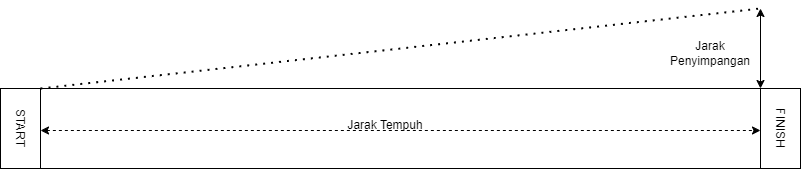
\includegraphics[scale=0.55]{gambar/program/Sudut Penyimpangan.png}
  % Keterangan gambar yang diinputkan
  \caption{Sistem Pengujian Kestabilan Motor Kursi Roda}
  % Label referensi dari gambar yang diinputkan
  \label{fig:PengujianKestabilanMotor}
\end{figure}

\begin{equation}
  \label{eq:sudut-error}
  Sudut Penyimpangan = \arctan \left ( \frac{Jarak Penyimpangan}{Jarak Tempuh} \right )
\end{equation}

\begin{description}[nolistsep]
  \item[Keterangan]
  \item[Sudut Penyimpangan] : Besar sudut penyimpangan gerak motor kursi roda (\textdegree)
  \item[Jarak Penyimpangan] : Jarak penyimpangan posisi akhir roda yang diukur dari posisi garis lurus jarak tempuh (cm)
  \item[Jarak Tempuh] : Lintasan garis lurus yang harus ditempuh oleh kursi roda (m)
\end{description}

\begin{longtable}{|ccc|c|}
  \caption{Pengujian Kestabilan Motor Kursi Roda Dengan Gerak Maju}
  \label{tbl:kestabilanmaju}\\
  \hline
  \multicolumn{1}{|c|}{\begin{tabular}[c]{@{}c@{}}Jarak \\ Tempuh\end{tabular}} & \multicolumn{1}{c|}{\begin{tabular}[c]{@{}c@{}}Jarak \\ Penyimpangan\end{tabular}} & \begin{tabular}[c]{@{}c@{}}Sudut\\ Penyimpangan\end{tabular} & \begin{tabular}[c]{@{}c@{}}Arah\\ Penyimpangan\end{tabular} \\ \hline
  \endfirsthead
  %
  \endhead
  %
  \multicolumn{1}{|c|}{10,34}                                                   & \multicolumn{1}{c|}{47}                                                            & 2,60\textdegree                                              & Kiri                                                        \\ \hline
  \multicolumn{1}{|c|}{10,50}                                                   & \multicolumn{1}{c|}{49}                                                            & 2,67\textdegree                                              & Kiri                                                        \\ \hline
  \multicolumn{1}{|c|}{10,74}                                                   & \multicolumn{1}{c|}{53}                                                            & 2,83\textdegree                                              & Kiri                                                        \\ \hline
  \multicolumn{1}{|c|}{10,53}                                                   & \multicolumn{1}{c|}{51}                                                            & 2,77\textdegree                                              & Kiri                                                        \\ \hline
  \multicolumn{1}{|c|}{10,62}                                                   & \multicolumn{1}{c|}{57}                                                            & 3,07\textdegree                                              & Kiri                                                        \\ \hline
  \multicolumn{3}{|c|}{Sudut Penyimpangan Rata - Rata}                                                                                                                                                                              & 2,788\textdegree                                            \\ \hline
  \end{longtable}

Tabel \ref{tbl:kestabilanmaju} menampilkan hasil pengujian kestabilan motor kursi roda dengan gerak maju. Pengujian ini dilakukan sebanyak 5 kali dengan jarak tempuh bervariasi dan lebih dari 10 meter. Hasil dari pengujian ini menunjukkan bahwa kursi roda cenderung bergerak kearah kiri dengan rata-rata sudut penyimpangan sebesar 2,788\textdegree.

\begin{longtable}{|ccc|c|}
  \caption{Pengujian Kestabilan Motor Kursi Roda Dengan Gerak Mundur}
  \label{tbl:kestabilanmundur}\\
  \hline
  \multicolumn{1}{|c|}{\begin{tabular}[c]{@{}c@{}}Jarak \\ Tempuh\end{tabular}} & \multicolumn{1}{c|}{\begin{tabular}[c]{@{}c@{}}Jarak \\ Penyimpangan\end{tabular}} & \begin{tabular}[c]{@{}c@{}}Sudut\\ Penyimpangan\end{tabular} & \begin{tabular}[c]{@{}c@{}}Arah\\ Penyimpangan\end{tabular} \\ \hline
  \endfirsthead
  %
  \endhead
  %
  \multicolumn{1}{|c|}{10,17}                                                   & \multicolumn{1}{c|}{102}                                                           & 5,73\textdegree                                              & Kanan                                                       \\ \hline
  \multicolumn{1}{|c|}{10,33}                                                   & \multicolumn{1}{c|}{96}                                                            & 5.31\textdegree                                              & Kanan                                                       \\ \hline
  \multicolumn{1}{|c|}{10,24}                                                   & \multicolumn{1}{c|}{91}                                                            & 5,08\textdegree                                              & Kanan                                                       \\ \hline
  \multicolumn{1}{|c|}{10,67}                                                   & \multicolumn{1}{c|}{107}                                                           & 5,73\textdegree                                              & Kanan                                                       \\ \hline
  \multicolumn{1}{|c|}{10,46}                                                   & \multicolumn{1}{c|}{103}                                                           & 5,62\textdegree                                              & Kanan                                                       \\ \hline
  \multicolumn{3}{|c|}{Sudut Penyimpangan Rata - Rata}                                                                                                                                                                              & 5,494\textdegree                                            \\ \hline
  \end{longtable}

  Tabel \ref{tbl:kestabilanmundur} menampilkan hasil pengujian kestabilan motor kursi roda dengan gerak mundur. Pengujian ini dilakukan sebanyak 5 kali dengan jarak tempuh bervariasi dan lebih dari 10 meter. Hasil dari pengujian ini menunjukkan bahwa kursi roda cenderung bergerak kearah kanan dengan rata-rata sudut penyimpangan sebesar 5,494\textdegree.